\documentclass[a4paper,10pt]{article}
\usepackage[T1]{fontenc}
\usepackage[utf8]{inputenc}
\usepackage[english]{babel}
\usepackage{lmodern}
\usepackage[top=1.6cm,bottom=1.8cm,left=1.9cm,right=1.9cm]{geometry}
\usepackage{titlesec,enumitem,xcolor,graphicx,lastpage,fancyhdr}
\usepackage{fontawesome5}
\usepackage[hidelinks]{hyperref}

\hypersetup{colorlinks=true,urlcolor=blue!70!black,linkcolor=blue!70!black}
\pagestyle{fancy}\fancyhf{}\renewcommand{\headrulewidth}{0pt}
\fancyfoot[C]{\small\color{gray}Page \thepage\ of \pageref{LastPage}}
\setlength{\parindent}{0pt}

\titleformat{\section}{\large\bfseries\color{blue!70!black}}{}{0em}{}[\vspace{-0.7em}\rule{\textwidth}{0.5pt}]
\titlespacing{\section}{0pt}{9pt}{5pt}
\setlist[itemize]{leftmargin=1.1em,itemsep=2pt,topsep=2pt,parsep=0pt}
\newcommand{\role}[4]{\vspace{3pt}\noindent\hspace{0.6em}\parbox[t]{0.38\textwidth}{\raggedright\textbf{#1}}\hfill\parbox[t]{0.58\textwidth}{\raggedleft\textit{#2}}\\{\textit{#3}\hfill\textit{#4}}\vspace{1pt}}

\begin{document}
\noindent
\begin{minipage}[t]{0.78\textwidth}
\vspace{0pt}
{\huge\bfseries Prabhavit Gupta}\\[8pt]
{\small \faPhone\ +39-351-610-7807 \quad \faEnvelope\ \href{mailto:prabhavitg@gmail.com}{prabhavitg@gmail.com} \quad \faLinkedin\ \href{https://www.linkedin.com/in/prabhavit/}{Linkedin} \quad \faMapMarker*\ Venice, Italy}
\end{minipage}\hfill
\begin{minipage}[t]{0.18\textwidth}
\vspace{0pt}\raggedleft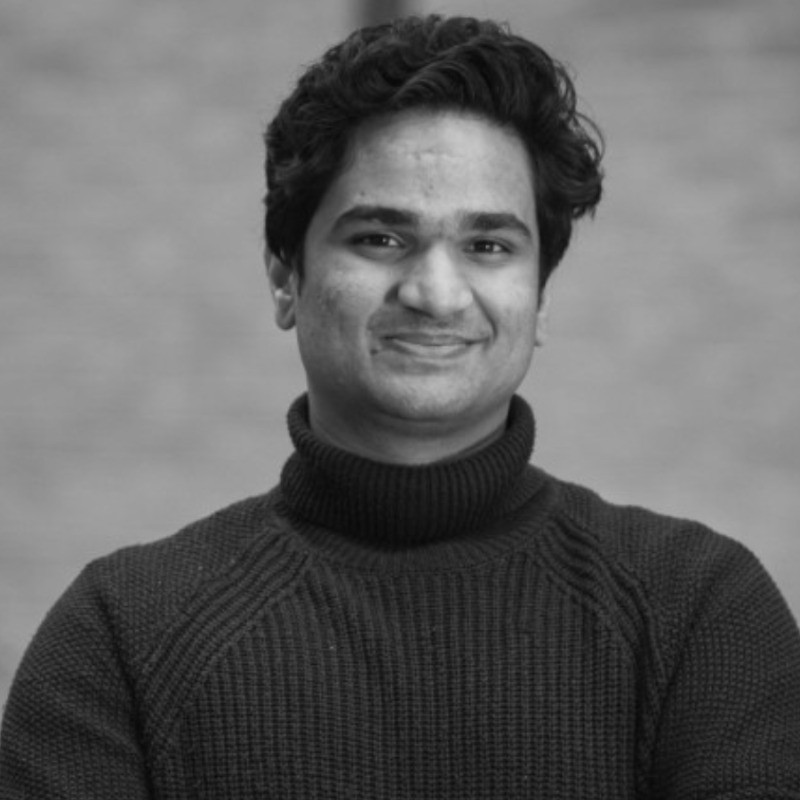
\includegraphics[width=2.3cm,height=2.3cm,keepaspectratio]{photo.jpg}
\end{minipage}

\section{Career Summary}
\begin{itemize}
\item Automation \& Robotics Engineer based in Veneto (Venice), holding dual degrees in Mechanical Engineering (B.E.) and Management Engineering (M.Sc., Politecnico di Milano).
\item Solid experience managing industrial automation and robotics integration projects from initial concept through system commissioning (messa in esercizio e collaudo).
\item Proficient in programming control algorithms and telemetry pipelines in Python and C++, with working knowledge of PLC logic (Siemens, Rockwell) and robotic workcells.
\item Proven capability in mechanical design (CAD/AutoCAD/Creo), supplier technical coordination, economic feasibility analysis, and Lean Manufacturing principles.
\end{itemize}

\section{Technical Skills}
\begin{itemize}
\item \textbf{Robotics \& Industrial Automation} -- Robotic Workcells, Kinematics, PLC Control Logic (Siemens TIA Portal, Rockwell), HMI/SCADA Interfaces, Fieldbus Networks (Profinet, Modbus)
\item \textbf{Software Development} -- Python, C++, Bash, Linux, SQL, ROS / Robotics Frameworks, Automated Verification Scripts, Git
\item \textbf{CAD \& Mechanical Design} -- 3D Modeling (AutoCAD, Creo, SolidWorks), Mechanical Systems Sizing, Pneumatic \& Electrical Schematics
\item \textbf{Project Management \& Lean} -- Technical Feasibility Studies, CAPEX/OPEX Analysis, Vendor Technical Management, Lean Manufacturing, Factory Acceptance (FAT/SAT)
\item \textbf{Testing \& Commissioning} -- Machinery Collaudo, Sensor Calibration, Root Cause Analysis, Technical Operating Procedures
\end{itemize}

\section{Visa \& Language}
\begin{itemize}
\item \textbf{Language} -- Italian (Conversational / Intermediate), English (Fluent / Professional), Hindi (Native)
\item \textbf{Work Authorization} -- European Long Term Residence Permit (No Visa Sponsorship required). Driving License (Patente B). Resident in Veneto (immediate availability for Noventa di Piave).
\end{itemize}

\section{Professional Experience}
\role{\href{https://flowspace.co}{FlowSpace.co}}{Automation \& Robotics Systems Lead}{London, UK / Remote}{Mar 2024 -- Ongoing}
\begin{itemize}
\item \textbf{Automation Project Engineering \& Delivery:}
\begin{itemize}[label=--]
\item Directed the technical architecture and delivery of distributed automated process systems, coordinating hardware interfaces and software deployments.
\item Developed high-reliability telemetry pipelines and control routines in Python and C++, evaluating cycle times and anomaly recovery.
\item Drafted comprehensive technical specifications, user requirements, and acceptance testing checklists for external technology vendors.
\end{itemize}
\item \textbf{Continuous Improvement \& Process Efficiency:}
\begin{itemize}[label=--]
\item Partnered with operations teams to streamline automated workflows, applying Lean concepts to eliminate throughput bottlenecks.
\item Ensured 99.9\% operational availability across active automated processes via proactive diagnostic monitoring and preventive maintenance protocols.
\end{itemize}
\item \textit{Tools: Python, C++, Linux, Docker, Industrial Networks, Git, Lean Tools}
\end{itemize}

\role{Urlink}{Systems Automation Engineer}{Milan, Italy}{Jul 2023 -- Feb 2024}
\begin{itemize}
\item Conducted on-site testing and commissioning (collaudo) of automated industrial machinery and robotic handling systems at manufacturing customer plants.
\item Verified PLC I/O configurations, safety interlocks, and sensor integrations adhering strictly to electrical schematics and CAD drawings.
\item Collaborated with suppliers and plant technicians to resolve mechanical and control logic discrepancies during equipment installation.
\end{itemize}

\role{UltraStrategy}{Automation Developer}{Remote, Germany}{Sep 2022 -- Jun 2023}
\begin{itemize}
\item Built automated data logging tools in Python monitoring industrial equipment operational parameters, cycle efficiency, and downtime trends.
\item Synthesized multi-stream machine sensor logs into structured performance analytics for quality and plant management.
\end{itemize}

\section{Education}
\role{Politecnico di Milano}{M.Sc. in Management Engineering (Digital Business \& ICT)}{Milan, Italy}{2020 -- 2023}
\role{Thapar Institute of Engineering and Technology}{B.E. in Mechanical Engineering}{Punjab, India}{2014 -- 2018}

\end{document}
